% ============================================================
%  DARWIN-PHOENIX — Main Paper
%  Compile: pdflatex PAPER.tex  (twice for cross-references)
%  Requires: newtxtext, newtxmath, booktabs, amsmath, hyperref, listings, geometry
% ============================================================
\documentclass[11pt,letterpaper]{article}

% --- Core packages ---
\usepackage[margin=1in]{geometry}
\usepackage{newtxtext}          % Modern Times Roman text (replaces obsolete mathptmx)
\usepackage{newtxmath}          % Matching Times math fonts
\usepackage[T1]{fontenc}
\usepackage[utf8]{inputenc}
\usepackage{microtype}          % Subtle typographic improvements (kerning, spacing)

% --- Math ---
\usepackage{amsmath,amssymb}

% --- Tables ---
\usepackage{booktabs}
\usepackage{array}
\usepackage{multirow}
\usepackage{xcolor}

% --- Figures ---
\usepackage{graphicx}
\usepackage[font=small,labelfont=bf,labelsep=period,
            justification=justified,singlelinecheck=false]{caption}
\usepackage{subcaption}

% --- Code listings ---
\usepackage{listings}
\lstset{
  basicstyle=\ttfamily\small,
  breaklines=true,
  breakatwhitespace=false,
  frame=single,
  backgroundcolor=\color{gray!7},
  rulecolor=\color{gray!35},
  xleftmargin=8pt,
  xrightmargin=8pt,
  showstringspaces=false,
  columns=flexible,
}

% --- Spacing ---
\usepackage{parskip}
\setlength{\parindent}{0pt}
\setlength{\parskip}{8pt plus 2pt minus 1pt}

% --- Section formatting ---
\usepackage{titlesec}
\titleformat{\section}{\large\bfseries}{\thesection.}{0.5em}{}
\titleformat{\subsection}{\normalsize\bfseries}{\thesubsection}{0.5em}{}
\titleformat{\subsubsection}{\normalsize\itshape\bfseries}{\thesubsubsection}{0.5em}{}
\titlespacing*{\section}      {0pt}{14pt plus 4pt minus 2pt}{6pt plus 2pt}
\titlespacing*{\subsection}   {0pt}{10pt plus 3pt minus 2pt}{4pt plus 1pt}
\titlespacing*{\subsubsection}{0pt}{8pt  plus 2pt minus 1pt}{3pt}

% --- Abstract styling ---
\usepackage{abstract}
\renewcommand{\abstractnamefont}{\normalfont\bfseries}
\renewcommand{\abstracttextfont}{\normalfont\small}
\setlength{\absleftindent}{0.5cm}
\setlength{\absrightindent}{0.5cm}

% --- Tight lists ---
\usepackage{enumitem}
\setlist{noitemsep, topsep=4pt, partopsep=0pt}

% --- Running headers ---
\usepackage{fancyhdr}
\pagestyle{fancy}
\fancyhf{}
\fancyhead[L]{\small\itshape DARWIN-PHOENIX: Behavioral Drift Under Adversarial Co-Evolution}
\fancyhead[R]{\small\itshape S.\ Yalamanchili}
\fancyfoot[C]{\small\thepage}
\renewcommand{\headrulewidth}{0.4pt}
\fancypagestyle{plain}{%
  \fancyhf{}%
  \fancyfoot[C]{\small\thepage}%
  \renewcommand{\headrulewidth}{0pt}}

% --- Compact fractions ---
\usepackage{nicefrac}

% --- Keywords command ---
\providecommand{\keywords}[1]{%
  \vspace{6pt}\noindent\textbf{Keywords:}\enspace\textit{#1}\vspace{2pt}}

% --- Hyperlinks (loaded last — standard LaTeX practice) ---
\usepackage[colorlinks=true,linkcolor=blue!70!black,
            citecolor=blue!70!black,urlcolor=blue!70!black,
            breaklinks=true]{hyperref}
\usepackage{xurl}               % Better URL line-breaking (supersedes url package)

% --- PDF metadata (machine readability — arXiv requirement) ---
\hypersetup{
  pdftitle   = {DARWIN-PHOENIX: Behavioral Drift Under Adversarial Co-Evolution
                Predicts Code Quality Degradation in LLM Code Generation},
  pdfauthor  = {Saketh Yalamanchili},
  pdfsubject = {cs.SE; cs.LG},
  pdfkeywords= {co-evolutionary AI, LLM code generation, behavioral fingerprinting,
                adversarial testing, antifragility, LangGraph, Qwen3-32B},
}

% ============================================================
\title{%
  \textbf{DARWIN-PHOENIX: Behavioral Drift Under Adversarial\\
  Co-Evolution Predicts Code Quality Degradation\\
  in LLM Code Generation}%
}

\author{%
  Saketh Yalamanchili\thanks{%
    Code, data, and full statistical reports available at
    \url{https://github.com/sakethyalamanchili/DARWIN-PHOENIX}}\\[2pt]
  \textit{M.S. Data Science \& Analytics}\\
  \textit{Florida Atlantic University}\\[2pt]
  \texttt{syalamanchil2025@fau.edu}%
}

\date{}

% ============================================================
\begin{document}
\maketitle
\thispagestyle{empty}

% ============================================================
\begin{abstract}
We introduce DARWIN-PHOENIX, a co-evolutionary LLM agent framework for
adversarially robust code generation, and present \textbf{behavioral
fingerprinting}---a novel TF-IDF cosine distance metric that quantifies
how much a generator agent's coding strategy shifts across adversarial
rounds.
Across three experiments on HumanEval+, our central finding is that
\textbf{behavioral drift strongly predicts code quality degradation}:
tasks with degraded outcomes exhibit $2.6\times$ greater maximum
fingerprint drift than successful ones (mean~0.240 vs.~0.092;
Kruskal-Wallis $p=0.0003$), and drift increases monotonically with
adversarial round number (Spearman $\rho=0.720$, $p<0.0001$).
This drift-quality tradeoff reveals a fundamental tension in adversarial
co-evolution: the generator's behavioral flexibility---necessary for
adaptation---is simultaneously a risk factor for quality regression when
drift overshoots the solution space.
Beyond fingerprinting, a pilot study across four conditions
($n=164$ tasks each) shows a consistent directional ordering in
degradation rates: full co-evolution (C,~6.7\%) $<$ frozen adversary
(D,~7.3\%) $<$ baseline (A,~9.8\%) $<$ static failure corpus
(B,~11.0\%), suggesting dynamic adversarial pressure reduces degradation
more effectively than static failure exposure.
A fault injection study ($n=300$ runs) further shows co-evolutionary
hardening produces faster recovery from hallucination faults
(Mann-Whitney $p=0.010$) and a larger advantage under context overflow
(+8.0~pp).
Together, these findings establish behavioral fingerprinting as a
principled tool for monitoring generator strategy stability, and motivate
a powered follow-up study to confirm the directional degradation
findings.
\end{abstract}

\keywords{co-evolutionary AI \and LLM code generation \and behavioral
fingerprinting \and adversarial testing \and antifragility \and LangGraph}

% ============================================================
\section{Introduction}

Large language model (LLM)-based code generation has achieved remarkable
benchmark performance, yet generated code remains brittle under adversarial
inputs, edge cases, and environmental faults. Standard approaches to
robustness rely on static techniques: post-hoc testing, retrieval-augmented
generation with failure examples, or prompt engineering. These approaches
treat robustness as a property to be imposed rather than evolved.

Antifragility, as defined by Taleb~\cite{taleb2012}, describes systems that
\emph{gain} from disorder---becoming stronger under stress rather than merely
resilient. We ask: can a code generation agent become antifragile through
sustained adversarial co-evolution? And critically: \textbf{how do we measure
whether it is adapting constructively versus drifting destructively?}

We introduce \textbf{DARWIN-PHOENIX}, a LangGraph-based framework in which:
\begin{itemize}
  \item \textbf{DARWIN} (generator) iteratively rewrites code to resist
        adversarial test failures.
  \item \textbf{PHOENIX} (breaker) generates targeted adversarial tests
        covering six attack vectors: integer overflow, empty input, type
        confusion, boundary values, unicode injection, and deep nesting.
\end{itemize}

The system runs for up to $N$ rounds, with the generator accumulating an
antifragility (AF) score based on pass rates, adversarial resistance, and
improvement trajectory. Our primary contribution is \textbf{behavioral
fingerprinting}: measuring TF-IDF cosine distance between Round~1 and
Round~$N$ code to detect when co-evolutionary pressure causes genuine strategy
drift versus surface-level refinement.

We compare four conditions:
\begin{itemize}
  \item \textbf{Condition A (baseline):} Single-pass generation, no adversarial
        testing.
  \item \textbf{Condition B (corpus):} Generator augmented with static failure
        corpus, no adversary.
  \item \textbf{Condition C (co-evolution):} Full DARWIN-PHOENIX co-evolutionary
        loop.
  \item \textbf{Condition D (frozen adversary):} Adversary generates tests only
        in Round~1, then freezes.
\end{itemize}

Our contributions are:
\begin{enumerate}
  \item \textbf{Behavioral fingerprinting method:} TF-IDF cosine distance as a
        round-by-round signal of generator strategy drift under adversarial
        pressure.
  \item \textbf{Drift-quality tradeoff:} Empirical evidence that large behavioral
        drift predicts code quality degradation ($p=0.0003$), revealing a
        fundamental design tension in co-evolutionary systems.
  \item \textbf{Pilot degradation evidence:} Consistent directional ordering
        C $<$ D $<$ A $<$ B across 656~runs, suggesting dynamic adversarial
        pressure outperforms static failure exposure.
  \item \textbf{Fault injection protocol:} Recovery measurement under
        hallucination, context overflow, and timeout faults, with a
        co-evolutionary advantage under hallucination recovery ($p=0.010$).
\end{enumerate}

% ============================================================
\section{Related Work}

\textbf{LLM Code Generation.}
Codex~\cite{chen2021}, AlphaCode~\cite{li2022}, and subsequent models achieve
high pass@$k$ on HumanEval~\cite{chen2021} and MBPP~\cite{austin2021}.
HumanEval+~\cite{liu2023} extends these benchmarks with adversarial test
augmentation, revealing that pass rates drop significantly under harder
evaluation. SWE-bench~\cite{jimenez2024} further challenges LLMs on real-world
GitHub issue resolution.

\textbf{Adversarial Testing.}
Fuzzing~\cite{bohme2021} and property-based testing~\cite{claessen2000} have
long been used to find software bugs. Recent work applies LLMs to test
generation~\cite{liu2023}, but typically in a single-pass, non-iterative
manner.

\textbf{Iterative Refinement.}
Self-repair~\cite{olausson2023}, Reflexion~\cite{shinn2023},
Self-Refine~\cite{madaan2023}, and execution feedback~\cite{chen2021} enable
LLMs to revise code based on test failures. These approaches use fixed test
suites; DARWIN-PHOENIX uses a co-evolving adversary that adapts to each code
version, creating a genuine arms race rather than a static evaluation loop.

\textbf{Co-evolutionary Systems.}
Red-teaming~\cite{perez2022} and Constitutional AI~\cite{bai2022} use
adversarial agents for alignment, not code quality. DARWIN-PHOENIX is the first
co-evolutionary system specifically designed for code antifragility measurement,
with behavioral fingerprinting providing a novel observability mechanism for
generator strategy evolution.

\textbf{Behavioral Analysis of LLMs.}
Prior work studies LLM behavioral consistency via output diversity and prompt
sensitivity. We extend this to \emph{within-task strategy drift under adversarial
pressure}---a novel measurement axis not previously quantified in code generation
settings.

\textbf{Antifragility in Software.}
Taleb's antifragility concept~\cite{taleb2012} describes systems that gain
strength from stressors. While applied to system architecture and resilience
engineering, it has not previously been operationalized as a measurable property
of LLM-generated code under adversarial pressure.

% ============================================================
\section{Methodology}

\subsection{System Architecture}

DARWIN-PHOENIX is implemented as a LangGraph \texttt{StateGraph} with seven
nodes executing in sequence each round. Figure~\ref{fig:architecture} shows
the full system architecture: solid edges denote LangGraph graph transitions;
dashed edges denote state data written by the Evolver and consumed by the
Generator and Breaker at the start of the next round.

\begin{figure}[htbp]
  \centering
  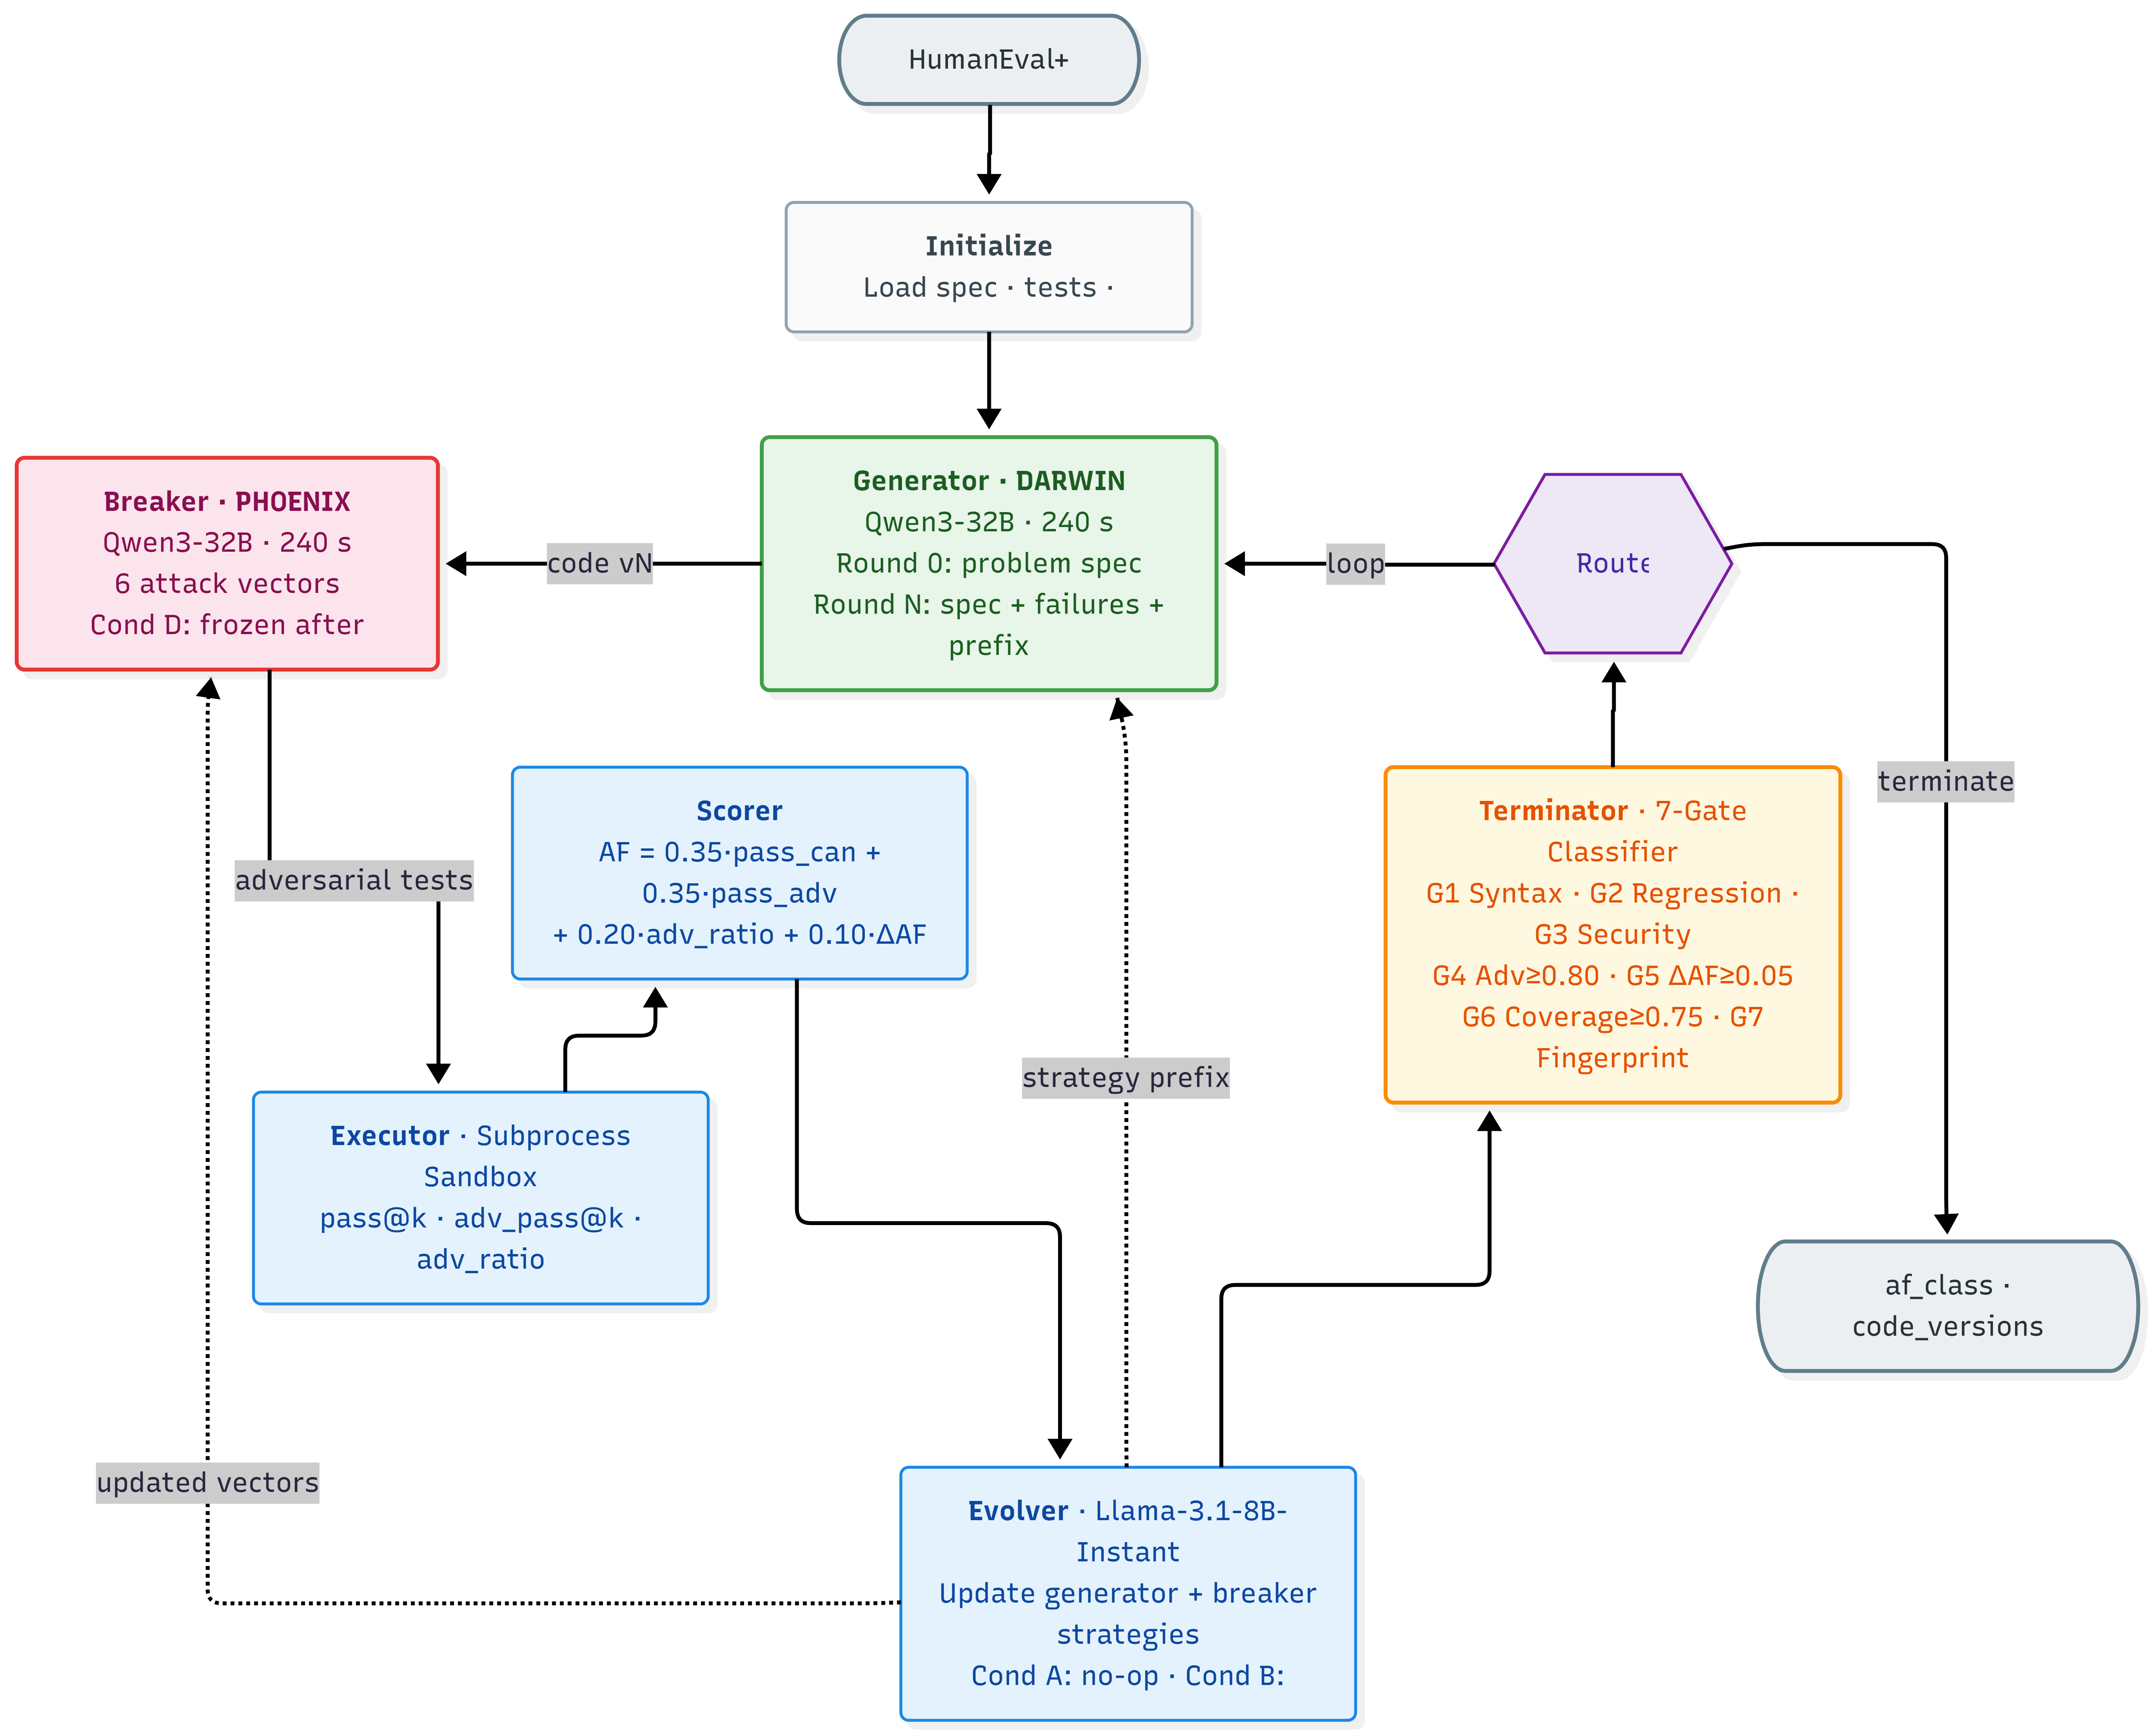
\includegraphics[width=\linewidth]{figures/fig_architecture.png}
  \caption{%
    \textbf{DARWIN-PHOENIX system architecture.}
    Seven nodes execute sequentially each round inside a LangGraph
    \texttt{StateGraph}.
    DARWIN (Generator, green) and PHOENIX (Breaker, red) form the
    co-evolutionary core; the Executor, Scorer, Evolver, and Terminator
    constitute the shared evaluation pipeline (blue).
    Solid arrows are LangGraph graph edges (execution order);
    dashed arrows are state updates carried forward to the next round.
    The Terminator applies a 7-gate deterministic classifier and routes
    to either a new generation round or the final state.
    Condition-specific behaviors are annotated per node
    (Cond~A: no adversary; Cond~B: static failure corpus;
     Cond~D: Breaker frozen after Round~1).%
  }
  \label{fig:architecture}
\end{figure}

\textbf{Initialize.} Loads task specification, canonical tests, and
condition-specific configuration from HumanEval+.

\textbf{Generator (DARWIN).} Produces or refines a Python function. Round~0
uses the full problem specification. Rounds~1+ receive the problem
specification, failed adversarial test cases, and a strategy prefix from the
evolver. Uses Qwen3-32B via OpenRouter with a 240-second wall-clock timeout
enforced by a \texttt{concurrent.futures.ThreadPoolExecutor} wrapper to prevent
thinking-bleed.

\textbf{Breaker (PHOENIX).} Generates adversarial test cases targeting the
current code using six attack vectors: integer overflow, empty input, type
confusion, boundary values, unicode injection, and deep nesting. In Condition~D,
the breaker strategy is frozen after Round~1. Uses Qwen3-32B.

\textbf{Executor.} Runs canonical and adversarial tests against the generated
code in a subprocess sandbox. Computes pass@$k$, adversarial pass@$k$,
adversarial ratio, and bug rate.

\textbf{Scorer.} Computes the antifragility (AF) score from execution results:
\begin{equation}
  \text{AF} =
    0.35\cdot\text{pass}_{\text{can}}
    + 0.35\cdot\text{pass}_{\text{adv}}
    + 0.20\cdot\text{adv\_ratio}
    + 0.10\cdot\Delta\text{AF}
  \label{eq:af}
\end{equation}
where $\text{pass}_{\text{can}}$ is canonical pass@$k$,
$\text{pass}_{\text{adv}}$ is adversarial pass@$k$,
$\text{adv\_ratio}$ is the fraction of tests that are adversarial, and
$\Delta\text{AF}$ is the round-over-round AF score delta.

\textbf{Evolver.} Uses Llama-3.1-8B-Instant to generate updated generator
defense heuristics and breaker attack vectors from current-round failures.
Condition~B injects failure corpus examples instead of adversarial test results.

\textbf{Terminator.} Applies a 7-gate deterministic classifier. Gates check:
syntax validity (G1), canonical test regression (G2), security vulnerabilities
via Bandit (G3), adversarial pass rate $\geq 0.80$ (G4), AF score improvement
$\geq 0.05$ (G5), branch coverage $\geq 0.75$ via Docker sandbox (G6), and
behavioral fingerprint change (G7). Outcome classes: \texttt{correct}
(passes G1--G5) or \texttt{degraded} (fails G1--G3).

\subsection{Antifragility Classification}

The terminator defines five outcome classes; only two were observed in practice
(Table~\ref{tab:classes}).

\begin{table}[htbp]
\centering
\caption{Terminator outcome classes and their observability in this study.}
\label{tab:classes}
\begin{tabular}{@{}lll@{}}
\toprule
\textbf{Class} & \textbf{Gate condition} & \textbf{Observed} \\
\midrule
\texttt{degraded}    & Fails G1, G2, or G3             & Yes (40--60\% of runs) \\
\texttt{correct}     & Passes G1--G3; no further progress & Yes (60--40\% of runs) \\
\texttt{antifragile} & All 7 gates pass (Docker required) & \textbf{Never} \\
\texttt{brittle}     & Planned; not implemented         & Never \\
\texttt{robust}      & Planned; not implemented         & Never \\
\bottomrule
\end{tabular}
\end{table}

\textbf{Note on antifragile non-occurrence.}
The G6 gate requires branch coverage measurement via a Docker sandbox
(\texttt{dp-sandbox} image). In this study, Docker was not deployed, causing
\texttt{edge\_coverage}~$=~0.0$ for all runs and making G6 permanently fail. As
a result, the \texttt{antifragile} class was structurally unreachable throughout
all experiments. We therefore measure \emph{degradation resistance} and
\emph{behavioral drift} as proxies for antifragility rather than direct
antifragile classification.

\subsection{LLM Configuration}

Generator (DARWIN) and Breaker (PHOENIX) use \textbf{Qwen3-32B} via OpenRouter.
The Evolver uses \textbf{Llama-3.1-8B-Instant} via OpenRouter for lightweight
strategy generation. Chain-of-thought thinking is disabled
(\texttt{enable\_thinking: False}) for Qwen3-32B to eliminate thinking-bleed.
A hard 240-second wall-clock timeout enforced via
\texttt{concurrent.futures.ThreadPoolExecutor} prevents indefinite streaming on
all calls. Timeout and rate-limit errors trigger exponential backoff with up to
6 outer retries (base 2.0~s, max 120~s per sleep); each \texttt{timed\_completion}
call has 3 inner retries.

\subsection{Behavioral Fingerprinting}

We measure generator behavioral drift using TF-IDF cosine distance between code
versions:
\begin{equation}
  d_{n} = \text{cosine\_distance}\!\bigl(\text{TF-IDF}(v_1),\,\text{TF-IDF}(v_n)\bigr)
  \label{eq:fingerprint}
\end{equation}
where $v_1$ is the Round~1 code and $v_n$ is the Round~$n$ code. Higher
distance indicates greater divergence in coding strategy---token-level
vocabulary, structure, variable naming---under adversarial pressure. Round~1
distance is always 0.0 by definition (baseline). The metric is computed using
scikit-learn's \texttt{TfidfVectorizer} with word-level tokenization preserving
code-specific tokens.

% ============================================================
\section{Experiments}

\subsection{Experiment~1: Behavioral Fingerprint Drift}

\textbf{Research Question.}
Does co-evolutionary adversarial pressure cause measurable, monotonic drift in
generator coding strategy? Does drift magnitude predict outcome quality?

\textbf{Design.}
50~HumanEval+ tasks, Condition~C only, minimum 2~rounds, up to 4~rounds.
TF-IDF cosine distance measured between Round~1 and all subsequent round code
versions.

\textbf{Metrics.}
Fingerprint distance per round; Spearman correlation of distance with round
number; Kruskal-Wallis test across rounds; maximum drift stratified by outcome
class.

\subsection{Experiment~2: Code Quality Across Conditions}

\textbf{Research Question.}
Does co-evolutionary adversarial pressure reduce degradation rates compared to
baseline and static failure exposure?

\textbf{Design.}
All 164~HumanEval+ tasks $\times$ 4~conditions (A, B, C, D) $= 656$~runs.
Up to 5~rounds per task with natural early termination.

\textbf{Metrics.}
Degradation rate (proportion of tasks with \texttt{af\_class}~$=$
\texttt{degraded}); AF score distribution; pairwise condition comparisons via
Fisher exact test; Cohen's $h$; power analysis.

\subsection{Experiment~3: Fault Recovery Under Injected Failures}

\textbf{Research Question.}
Does co-evolutionary hardening improve recovery from simulated production faults?

\textbf{Design.}
50~tasks $\times$ 2~conditions (A, C) $\times$ 3~fault types $= 300$~runs.

\textbf{Fault types:}
\begin{itemize}
  \item \emph{Hallucination:} Breaker generates semantically plausible but
        incorrect expected outputs, testing resistance to misleading test oracles.
  \item \emph{Context overflow:} Extremely long inputs near token limits, testing
        boundary handling.
  \item \emph{Timeout:} Injected latency forcing the executor to terminate early.
\end{itemize}

\textbf{Metrics.}
Recovery rate (binary: did the system recover to passing state); recovery steps;
Mann-Whitney U on step distributions; Kruskal-Wallis across fault types.

% ============================================================
\section{Results}
\label{sec:results}

\subsection{Behavioral Fingerprint Drift}

Round has a highly significant effect on fingerprint distance
(Kruskal-Wallis $H = 95.112$, $p < 0.0001$; Figure~\ref{fig:fingerprint}, left).
Distance increases monotonically with round number (Spearman $\rho = 0.720$,
$p < 0.0001$), confirming that sustained adversarial pressure causes the generator
to progressively diverge from its initial coding strategy. 96.8\% of distance
measurements at rounds~2+ are non-zero, ruling out measurement noise.

\textbf{Critical finding.}
Tasks classified as \texttt{degraded} exhibit $\mathbf{2.6\times}$
\textbf{greater maximum fingerprint drift} than \texttt{correct} tasks
(mean~$0.240$ vs.~$0.092$; Kruskal-Wallis $p = 0.0003$). Large strategy shifts
under adversarial pressure---while indicating responsiveness---frequently
overshoot the solution space and produce functionally degraded code. This
identifies a \textbf{drift-quality tradeoff}: behavioral flexibility is both
the source of adaptability and the primary risk factor for regression.

This finding has direct system design implications: adversarial pressure should
be calibrated to encourage local refinement rather than global strategy
replacement. Trajectory-aware termination that detects excessive drift and rolls
back to the last high-quality version is a natural mitigation.

\begin{table}[htbp]
\centering
\caption{TF-IDF fingerprint distance by round ($n=50$ tasks, Condition~C).}
\label{tab:fingerprint}
\begin{tabular}{@{}rrrrrr@{}}
\toprule
\textbf{Round} & \textbf{N} & \textbf{Mean} & \textbf{SD}
               & \textbf{Median} & \textbf{Range} \\
\midrule
1 (baseline) & 49 & 0.000 & 0.000 & 0.000 & 0.000--0.000 \\
2            & 42 & 0.162 & 0.115 & 0.148 & 0.000--0.442 \\
3            & 31 & 0.174 & 0.115 & 0.132 & 0.000--0.440 \\
4            & 22 & 0.201 & 0.151 & 0.156 & 0.042--0.614 \\
\bottomrule
\end{tabular}
\end{table}

\begin{figure}[htbp]
  \centering
  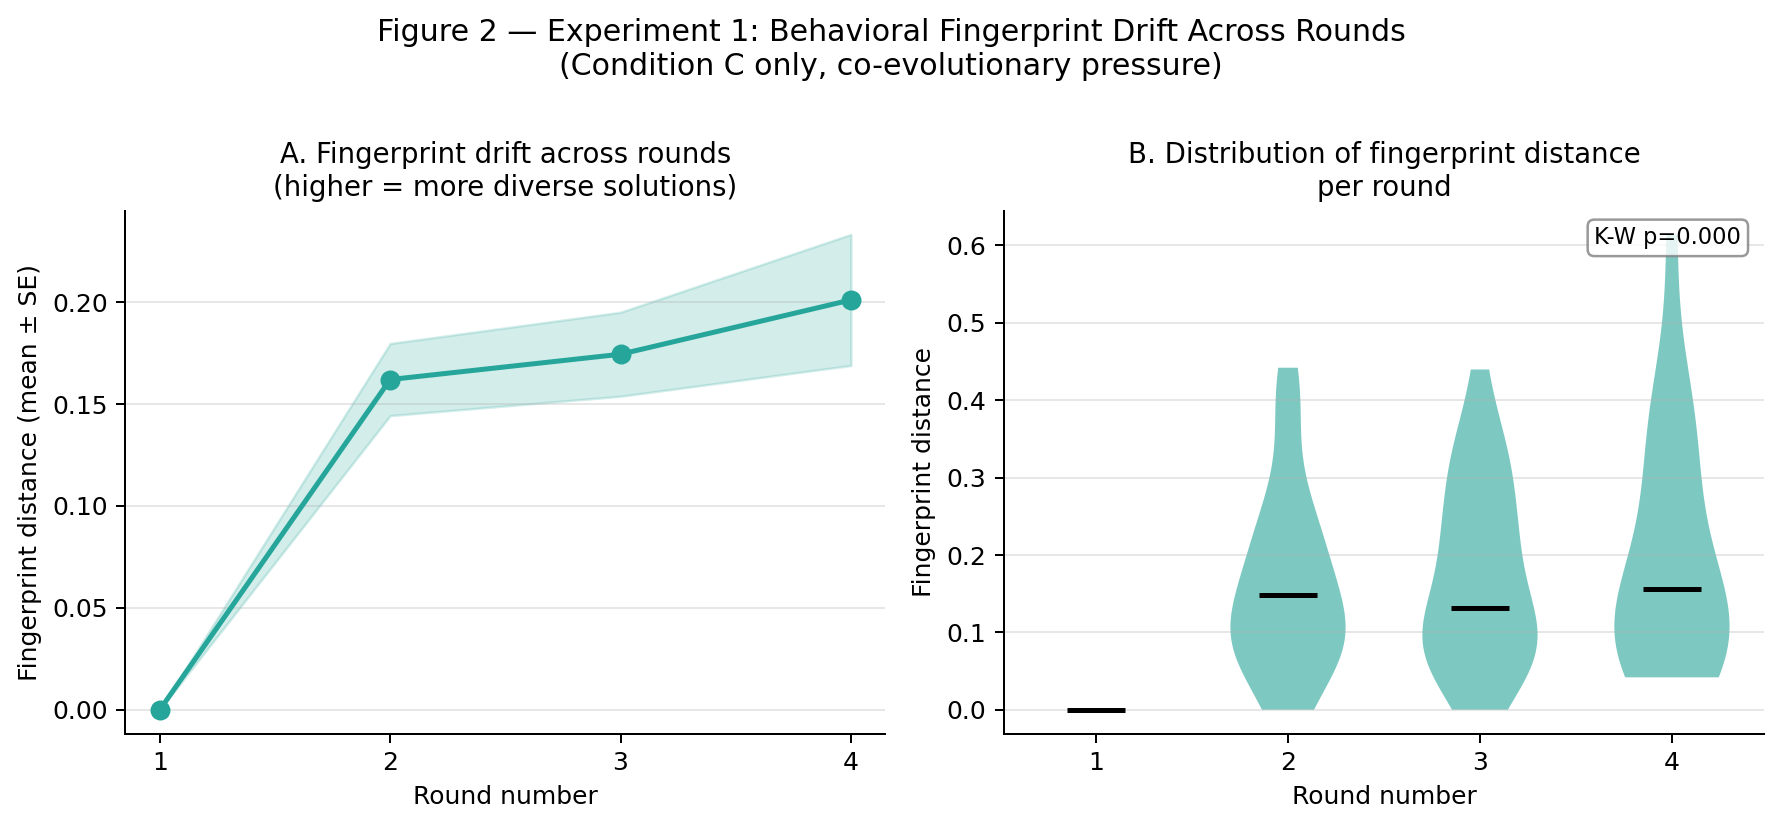
\includegraphics[width=0.95\linewidth]{figures/fig1_fingerprint.png}
  \caption{%
    \textbf{Experiment~1 --- Behavioral Fingerprint Drift.}
    (Left) Mean TF-IDF cosine distance per round ($\pm$SE); distance increases
    monotonically ($\rho=0.720$, $p<0.0001$).
    (Right) Per-round distribution (violin); spread grows with each round.
    Degraded-outcome tasks show $2.6\times$ greater max drift than
    correct-outcome tasks ($p=0.0003$).%
  }
  \label{fig:fingerprint}
\end{figure}

\subsection{Code Quality Across Conditions}

The ordering C $<$ D $<$ A $<$ B is monotonically consistent with the hypothesis
that dynamic adversarial pressure drives degradation resistance
(Figure~\ref{fig:quality}, center). Co-evolution (C) achieves the lowest
degradation rate (6.7\%), followed by frozen adversary (D,~7.3\%), baseline
(A,~9.8\%), and failure corpus (B,~11.0\%).

The pairwise Fisher exact test between C and B (primary hypothesis, one-sided)
yields OR~$= 0.58$, $p = 0.121$. This directional effect (Cohen's $h = 0.151$,
small) is consistent across all condition pairs but does not reach conventional
significance at $\alpha = 0.05$. A Kruskal-Wallis test on AF scores across all
four conditions approaches significance ($H = 7.537$, $p = 0.057$), providing
convergent evidence for a condition effect on generator quality. A power analysis
indicates the study is underpowered (49\%) to detect the observed effect;
approximately 342~tasks per condition would achieve 80\% power. These results
constitute \textbf{pilot evidence} warranting a powered follow-up study.

Notably, failure corpus augmentation (B) performs \emph{worse} than baseline (A),
suggesting static failure examples without adaptive pressure introduce
distributional bias or over-constrain the generator's solution space.

\begin{table}[htbp]
\centering
\caption{Outcome distribution and AF score by condition ($n = 164$ tasks each).}
\label{tab:quality}
\begin{tabular}{@{}lrrrrr@{}}
\toprule
\textbf{Condition} & \textbf{N} & \textbf{Correct} & \textbf{Degraded}
                   & \textbf{Degraded\%} & \textbf{Mean AF} \\
\midrule
A --- Baseline  & 164 & 148 & 16 & 9.8\%          & 0.048 \\
B --- Corpus    & 164 & 146 & 18 & 11.0\%         & 0.025 \\
C --- Co-Evol   & 164 & 153 & 11 & \textbf{6.7\%} & 0.024 \\
D --- Frozen    & 164 & 152 & 12 & 7.3\%          & 0.019 \\
\bottomrule
\end{tabular}
\end{table}

\begin{figure}[htbp]
  \centering
  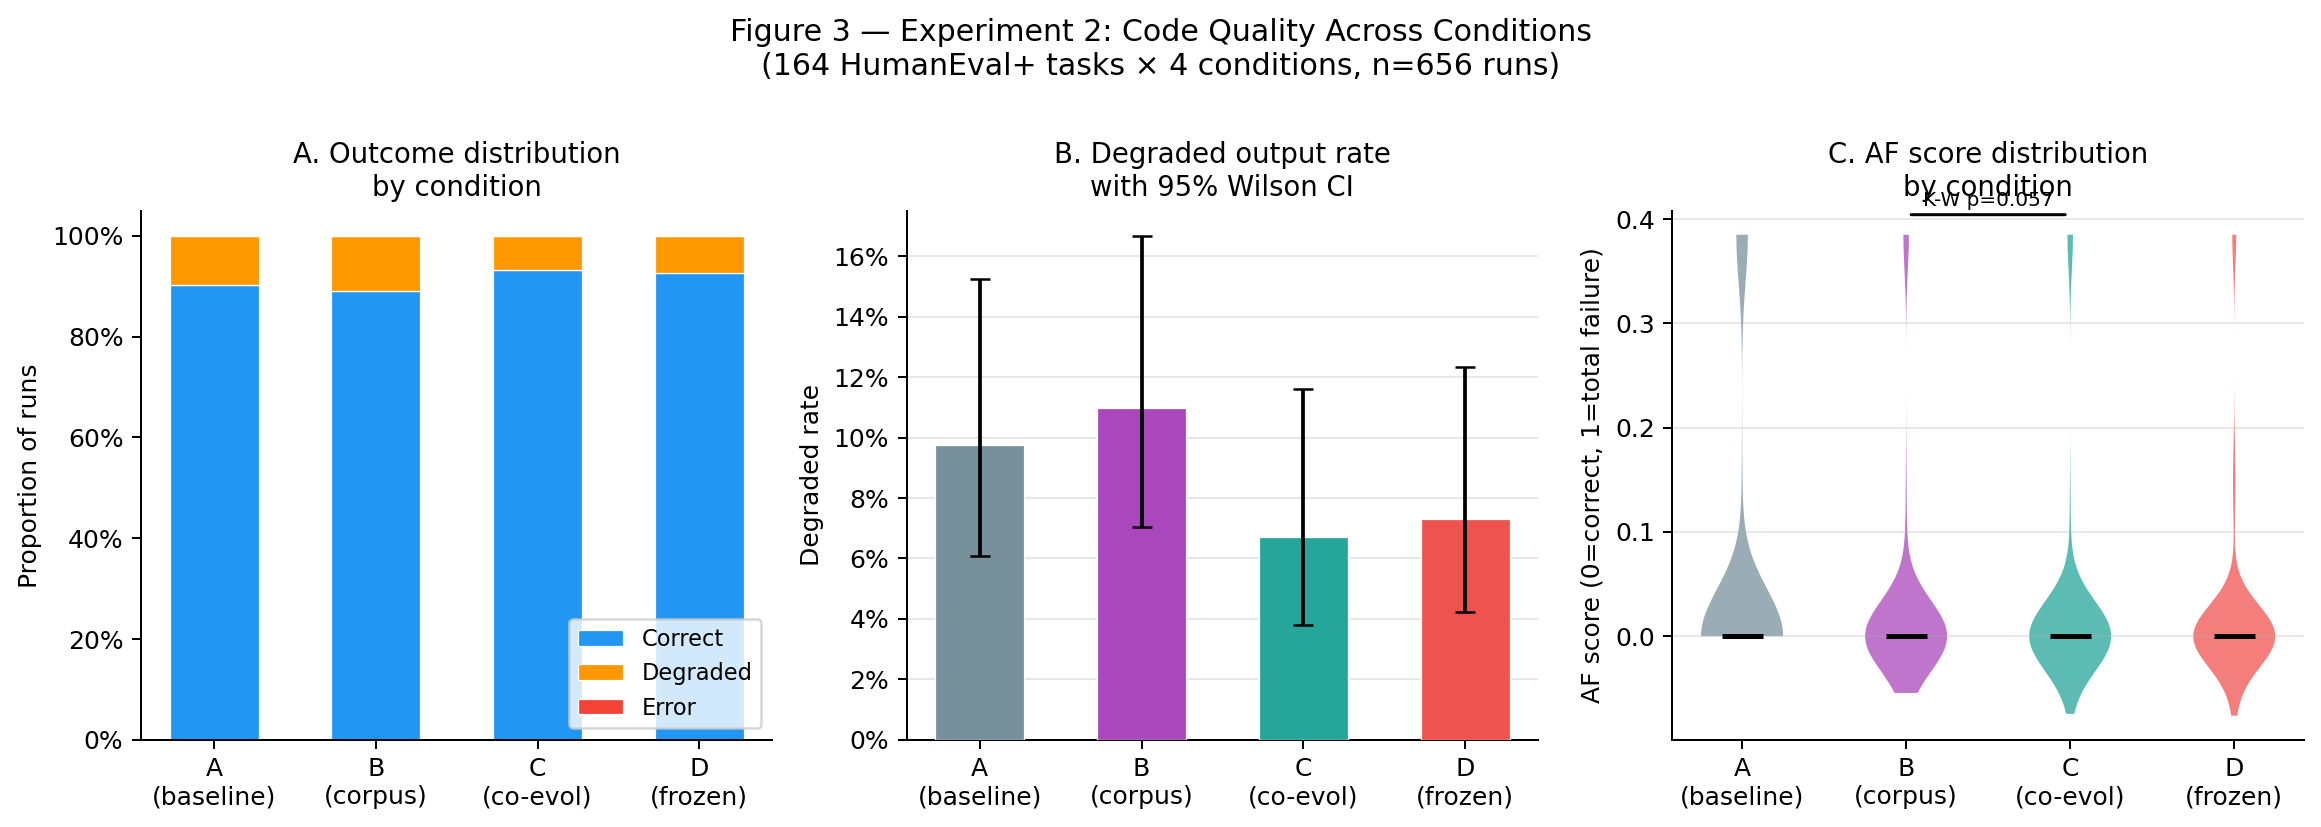
\includegraphics[width=0.95\linewidth]{figures/fig2_quality.png}
  \caption{%
    \textbf{Experiment~2 --- Code Quality Across Conditions.}
    (Left) Outcome distribution (correct / degraded) per condition.
    (Center) Degradation rate with 95\% Wilson confidence intervals; ordering
    C $<$ D $<$ A $<$ B is monotonically consistent.
    (Right) AF score distribution across conditions.%
  }
  \label{fig:quality}
\end{figure}

\subsection{Fault Recovery Under Injected Failures}

Co-evolutionary hardening (C) achieves a 3.3~percentage-point overall recovery
advantage (82.7\% vs.\ 79.3\%; Fisher exact $p = 0.278$; Cohen $h = 0.085$,
negligible overall effect; Figure~\ref{fig:recovery}, right). The largest
differential occurs for context overflow faults ($+8.0$~pp, Cohen $h = 0.209$,
small effect), suggesting co-evolutionary pressure specifically improves boundary
and edge-case handling.

Fault type significantly moderates recovery difficulty (Kruskal-Wallis on
recovery steps: $H = 10.498$, $p = 0.005$). Context overflow faults require
significantly more recovery steps (mean~1.37) than hallucination (1.17) or
timeout (1.17) faults, indicating context overflow presents the most
structurally complex failure mode.

The clearest co-evolutionary signal: \textbf{hallucination fault recovery step
distributions} differ significantly between conditions (Mann-Whitney $U = 903$,
$p = 0.010$), with Condition~C showing a more efficient step distribution despite
identical medians (both~1.0). Co-evolutionary hardening reduces recovery tail
length for hallucination faults---the rate difference is modest (+4.0~pp) but
the generator reaches recovery more consistently in fewer total attempts.

\begin{table}[htbp]
\centering
\caption{Recovery rates by condition and fault type ($n = 50$ runs per cell).}
\label{tab:recovery}
\begin{tabular}{@{}lrrrr@{}}
\toprule
\textbf{Fault Type} & \textbf{Cond A} & \textbf{Cond C}
                    & \textbf{$\Delta$} & \textbf{Cohen $h$} \\
\midrule
Hallucination    & 76.0\% & 80.0\% & $+4.0$~pp & 0.097  \\
Context overflow & 78.0\% & 86.0\% & $+8.0$~pp & 0.209  \\
Timeout          & 84.0\% & 82.0\% & $-2.0$~pp & $-0.053$ \\
\midrule
\textbf{Overall} & \textbf{79.3\%} & \textbf{82.7\%}
                 & $\mathbf{+3.3}$~\textbf{pp} & \textbf{0.085} \\
\bottomrule
\end{tabular}
\end{table}

\begin{figure}[htbp]
  \centering
  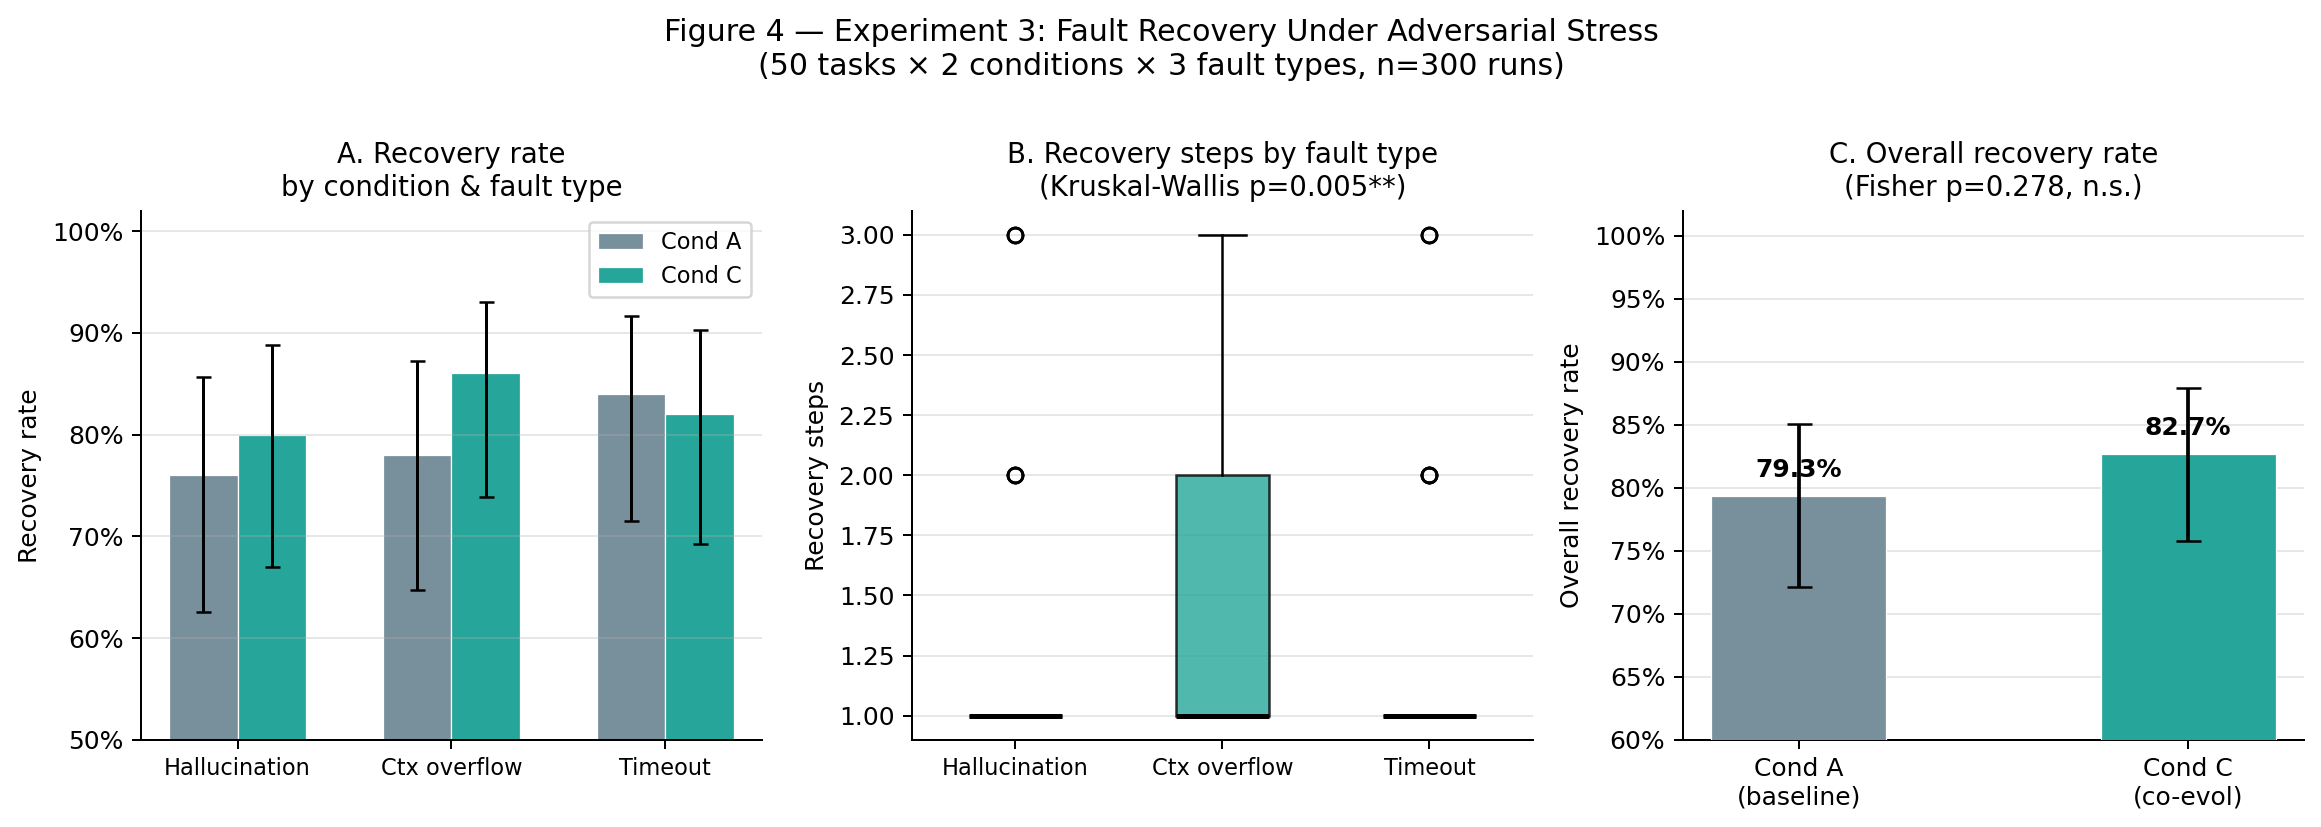
\includegraphics[width=0.95\linewidth]{figures/fig3_recovery.png}
  \caption{%
    \textbf{Experiment~3 --- Fault Recovery Under Injected Failures.}
    (Left) Recovery rates by condition $\times$ fault type with 95\% Wilson CIs.
    (Center) Recovery steps distribution (recovered runs only);
    hallucination step distributions differ significantly between conditions
    (Mann-Whitney $U=903$, $p=0.010$).
    (Right) Overall recovery rate comparison (A vs.\ C).%
  }
  \label{fig:recovery}
\end{figure}

% ============================================================
\section{Discussion}

\subsection{The Drift-Quality Tradeoff}

The central finding of this work is a fundamental tension in adversarial
co-evolution: the generator's behavioral flexibility---essential for adapting to
adversarial pressure---is simultaneously the primary predictor of quality
degradation. Tasks with high maximum drift (mean~0.240) degrade $2.6\times$ more
often than low-drift tasks (mean~0.092).

This has a clear mechanistic interpretation: when PHOENIX generates aggressive,
novel attack vectors, DARWIN responds by exploring distant regions of code space.
In some cases this exploration finds a better solution; in many cases it abandons
the correct solution structure entirely. The monotonic increase in drift across
rounds ($\rho = 0.720$) confirms this is not a one-time perturbation but a
cumulative drift process.

The practical implication is concrete: co-evolutionary systems need \textbf{drift
budgets}---a maximum tolerated distance from Round~1 code beyond which the system
rolls back rather than continuing to evolve. Behavioral fingerprinting provides
the measurement infrastructure for this mechanism.

\subsection{Dynamic vs.\ Static Adversarial Pressure}

The ordering C $<$ D $<$ A $<$ B in Experiment~2 reveals a nuanced picture.
Full co-evolution (C) outperforms frozen adversary (D), confirming that ongoing
adaptive pressure matters. Both adversarial conditions outperform baseline (A).
Most strikingly, static failure corpus (B) performs worst---suggesting curated
failure examples without live pressure introduce distributional overfitting,
constraining the generator toward known failure modes rather than genuinely
hardening it.

This ordering is consistent across all four conditions with no reversals---a
strong pattern for a pilot study, even absent individual pairwise significance.

\subsection{Fault-Type Sensitivity}

Context overflow faults are uniquely challenging: most recovery steps, largest
C-vs-A differential ($+8.0$~pp). Co-evolutionary hardening specifically targets
boundary-handling behaviors, consistent with PHOENIX's active focus on
\texttt{boundary\_values} and \texttt{deep\_nesting} attack vectors. Timeout
faults show negligible C-vs-A difference, consistent with timeout recovery being
architecturally independent of code quality.

The hallucination recovery step-distribution advantage ($p = 0.010$) despite a
modest rate advantage suggests co-evolutionary hardening builds resistance to
misleading test oracle signals---an important property for production deployment
where ground-truth labels are noisy.

\subsection{Limitations}

\begin{enumerate}

\item \textbf{Antifragile class unreachable.}
The G6 coverage gate requires a Docker sandbox (\texttt{dp-sandbox}) that was
not deployed in this study. All runs produced \texttt{edge\_coverage}~$= 0.0$,
making \texttt{antifragile} classification structurally impossible. We measure
degradation resistance and behavioral drift as indirect proxies.

\item \textbf{Underpowered primary test.}
The C-vs-B comparison (Fisher $p = 0.121$) does not reach significance at
$\alpha = 0.05$. A fully powered study requires approximately 342~tasks per
condition vs.\ our 164. The current results constitute directional pilot
evidence.

\item \textbf{Two models, not one.}
Generator and Breaker use Qwen3-32B; Evolver uses Llama-3.1-8B-Instant.
Observed outcomes reflect this specific combination and may not generalize to
other model pairings.

\item \textbf{HumanEval+ scope.}
Results are limited to short, self-contained Python functions. Complex
multi-file codebases may exhibit different dynamics.

\item \textbf{Behavioral fingerprinting proxy.}
TF-IDF cosine distance captures token-level vocabulary drift, not semantic
drift. Two semantically equivalent but syntactically different implementations
would register high distance. Semantic fingerprinting via code embeddings is a
natural extension.

\item \textbf{Intermediate failures in Experiment~1.}
13 of 50 tasks produced \texttt{ERROR} outcomes on at least one attempt before
eventually succeeding on retry. All 50 tasks have valid final fingerprint
records; these errors reflect API instability during collection, not final data
loss.

\end{enumerate}

% ============================================================
\section{Conclusion}

We present DARWIN-PHOENIX, a co-evolutionary LLM code generation framework, and
introduce \textbf{behavioral fingerprinting} as a novel measurement tool for
generator strategy drift under adversarial pressure. Our central empirical
finding is a drift-quality tradeoff: large behavioral drift under co-evolutionary
pressure strongly and significantly predicts code quality degradation
($\rho = 0.720$, $p < 0.0001$; $2.6\times$ drift ratio, $p = 0.0003$). This
establishes behavioral fingerprinting as a principled observability mechanism for
co-evolutionary systems.

Beyond fingerprinting, pilot evidence across 656~runs shows a consistent
directional ordering (C $<$ D $<$ A $<$ B) suggesting dynamic adversarial
pressure outperforms both static failure exposure and no adversary, though a
powered study ($n \geq 342$~tasks per condition) is required for definitive
confirmation. Fault injection results show co-evolutionary hardening produces
faster hallucination recovery ($p = 0.010$) and a larger boundary-fault
advantage ($+8.0$~pp).

These results motivate three concrete directions for future work:
\begin{enumerate}
  \item \textbf{Powered replication} with $n \geq 342$~tasks per condition and
        Docker-enabled coverage measurement to unlock the full 7-gate
        classification system.
  \item \textbf{Drift control mechanisms}---trajectory-aware termination using
        fingerprint distance as a rollback signal.
  \item \textbf{Semantic fingerprinting} using code embeddings to detect strategy
        drift at the semantic rather than token level.
\end{enumerate}

All code, data, and full statistical reports are available in the accompanying
repository at \url{https://github.com/sakethyalamanchili/DARWIN-PHOENIX}.

% ============================================================
\begin{thebibliography}{99}

\bibitem{taleb2012}
N.~N. Taleb,
\textit{Antifragile: Things That Gain from Disorder}.
Random House, 2012.

\bibitem{chen2021}
M.~Chen, J.~Tworek, H.~Jun, Q.~Yuan, H.~P.~O. Pinto, J.~Kaplan,
\textit{et~al.},
``Evaluating large language models trained on code,''
\textit{arXiv preprint arXiv:2107.03374}, 2021.

\bibitem{li2022}
Y.~Li, D.~Choi, J.~Chung, N.~Kushman, J.~Schrittwieser, R.~Leblond,
\textit{et~al.},
``Competition-level code generation with AlphaCode,''
\textit{Science}, vol.~378, no.~6624, pp.~1092--1097, 2022.

\bibitem{liu2023}
J.~Liu, C.~S. Xia, Y.~Wang, and L.~Zhang,
``Is your code generated by ChatGPT really correct? Rigorous evaluation
of large language models for code generation,''
in \textit{Advances in Neural Information Processing Systems (NeurIPS)},
vol.~36, 2023.

\bibitem{shinn2023}
N.~Shinn, F.~Cassano, A.~Gopinath, K.~Narasimhan, and S.~Yao,
``Reflexion: Language agents with verbal reinforcement learning,''
in \textit{Advances in Neural Information Processing Systems (NeurIPS)},
vol.~36, 2023.

\bibitem{olausson2023}
T.~X. Olausson, J.~P. Inala, C.~Wang, J.~Gao, and A.~Solar-Lezama,
``Is self-repair a silver bullet for code generation?''
in \textit{Proc. International Conference on Learning Representations (ICLR)},
2024.

\bibitem{perez2022}
E.~Perez, S.~Huang, F.~Song, T.~Cai, R.~Ring, J.~Aslanides,
\textit{et~al.},
``Red teaming language models with language models,''
\textit{arXiv preprint arXiv:2202.03286}, 2022.

\bibitem{bai2022}
Y.~Bai, A.~Jones, K.~Ndousse, A.~Askell, A.~Chen, N.~DasSarma,
\textit{et~al.},
``Constitutional AI: Harmlessness from AI feedback,''
\textit{arXiv preprint arXiv:2212.08073}, 2022.

\bibitem{claessen2000}
K.~Claessen and J.~Hughes,
``QuickCheck: A lightweight tool for random testing of Haskell programs,''
in \textit{Proc. ACM SIGPLAN International Conference on Functional
Programming (ICFP)}, pp.~268--279, 2000.

\bibitem{bohme2021}
M.~B\"{o}hme, C.~Cadar, and A.~Roychoudhury,
``Fuzzing: Challenges and reflections,''
\textit{IEEE Software}, vol.~38, no.~3, pp.~79--86, 2021.

\bibitem{austin2021}
J.~Austin, A.~Odena, M.~Nye, M.~Bosma, H.~Michalewski, D.~Dohan,
\textit{et~al.},
``Program synthesis with large language models,''
\textit{arXiv preprint arXiv:2108.07732}, 2021.

\bibitem{jimenez2024}
C.~E. Jimenez, J.~Yang, A.~Wettig, S.~Yao, K.~Pei, O.~Press,
and K.~Narasimhan,
``SWE-bench: Can language models resolve real-world GitHub issues?''
in \textit{Proc. International Conference on Learning Representations (ICLR)},
2024.

\bibitem{madaan2023}
A.~Madaan, N.~Tandon, P.~Gupta, S.~Hallinan, L.~Gao, S.~Wiegreffe,
\textit{et~al.},
``Self-refine: Iterative refinement with self-feedback,''
in \textit{Advances in Neural Information Processing Systems (NeurIPS)},
vol.~36, 2023.

\end{thebibliography}

% ============================================================
\appendix

\section{Experimental Figures}

Figures~\ref{fig:fingerprint}, \ref{fig:quality}, and \ref{fig:recovery} appear
inline in Section~\ref{sec:results}. The combined one-page summary is shown
below.

\begin{figure}[htbp]
  \centering
  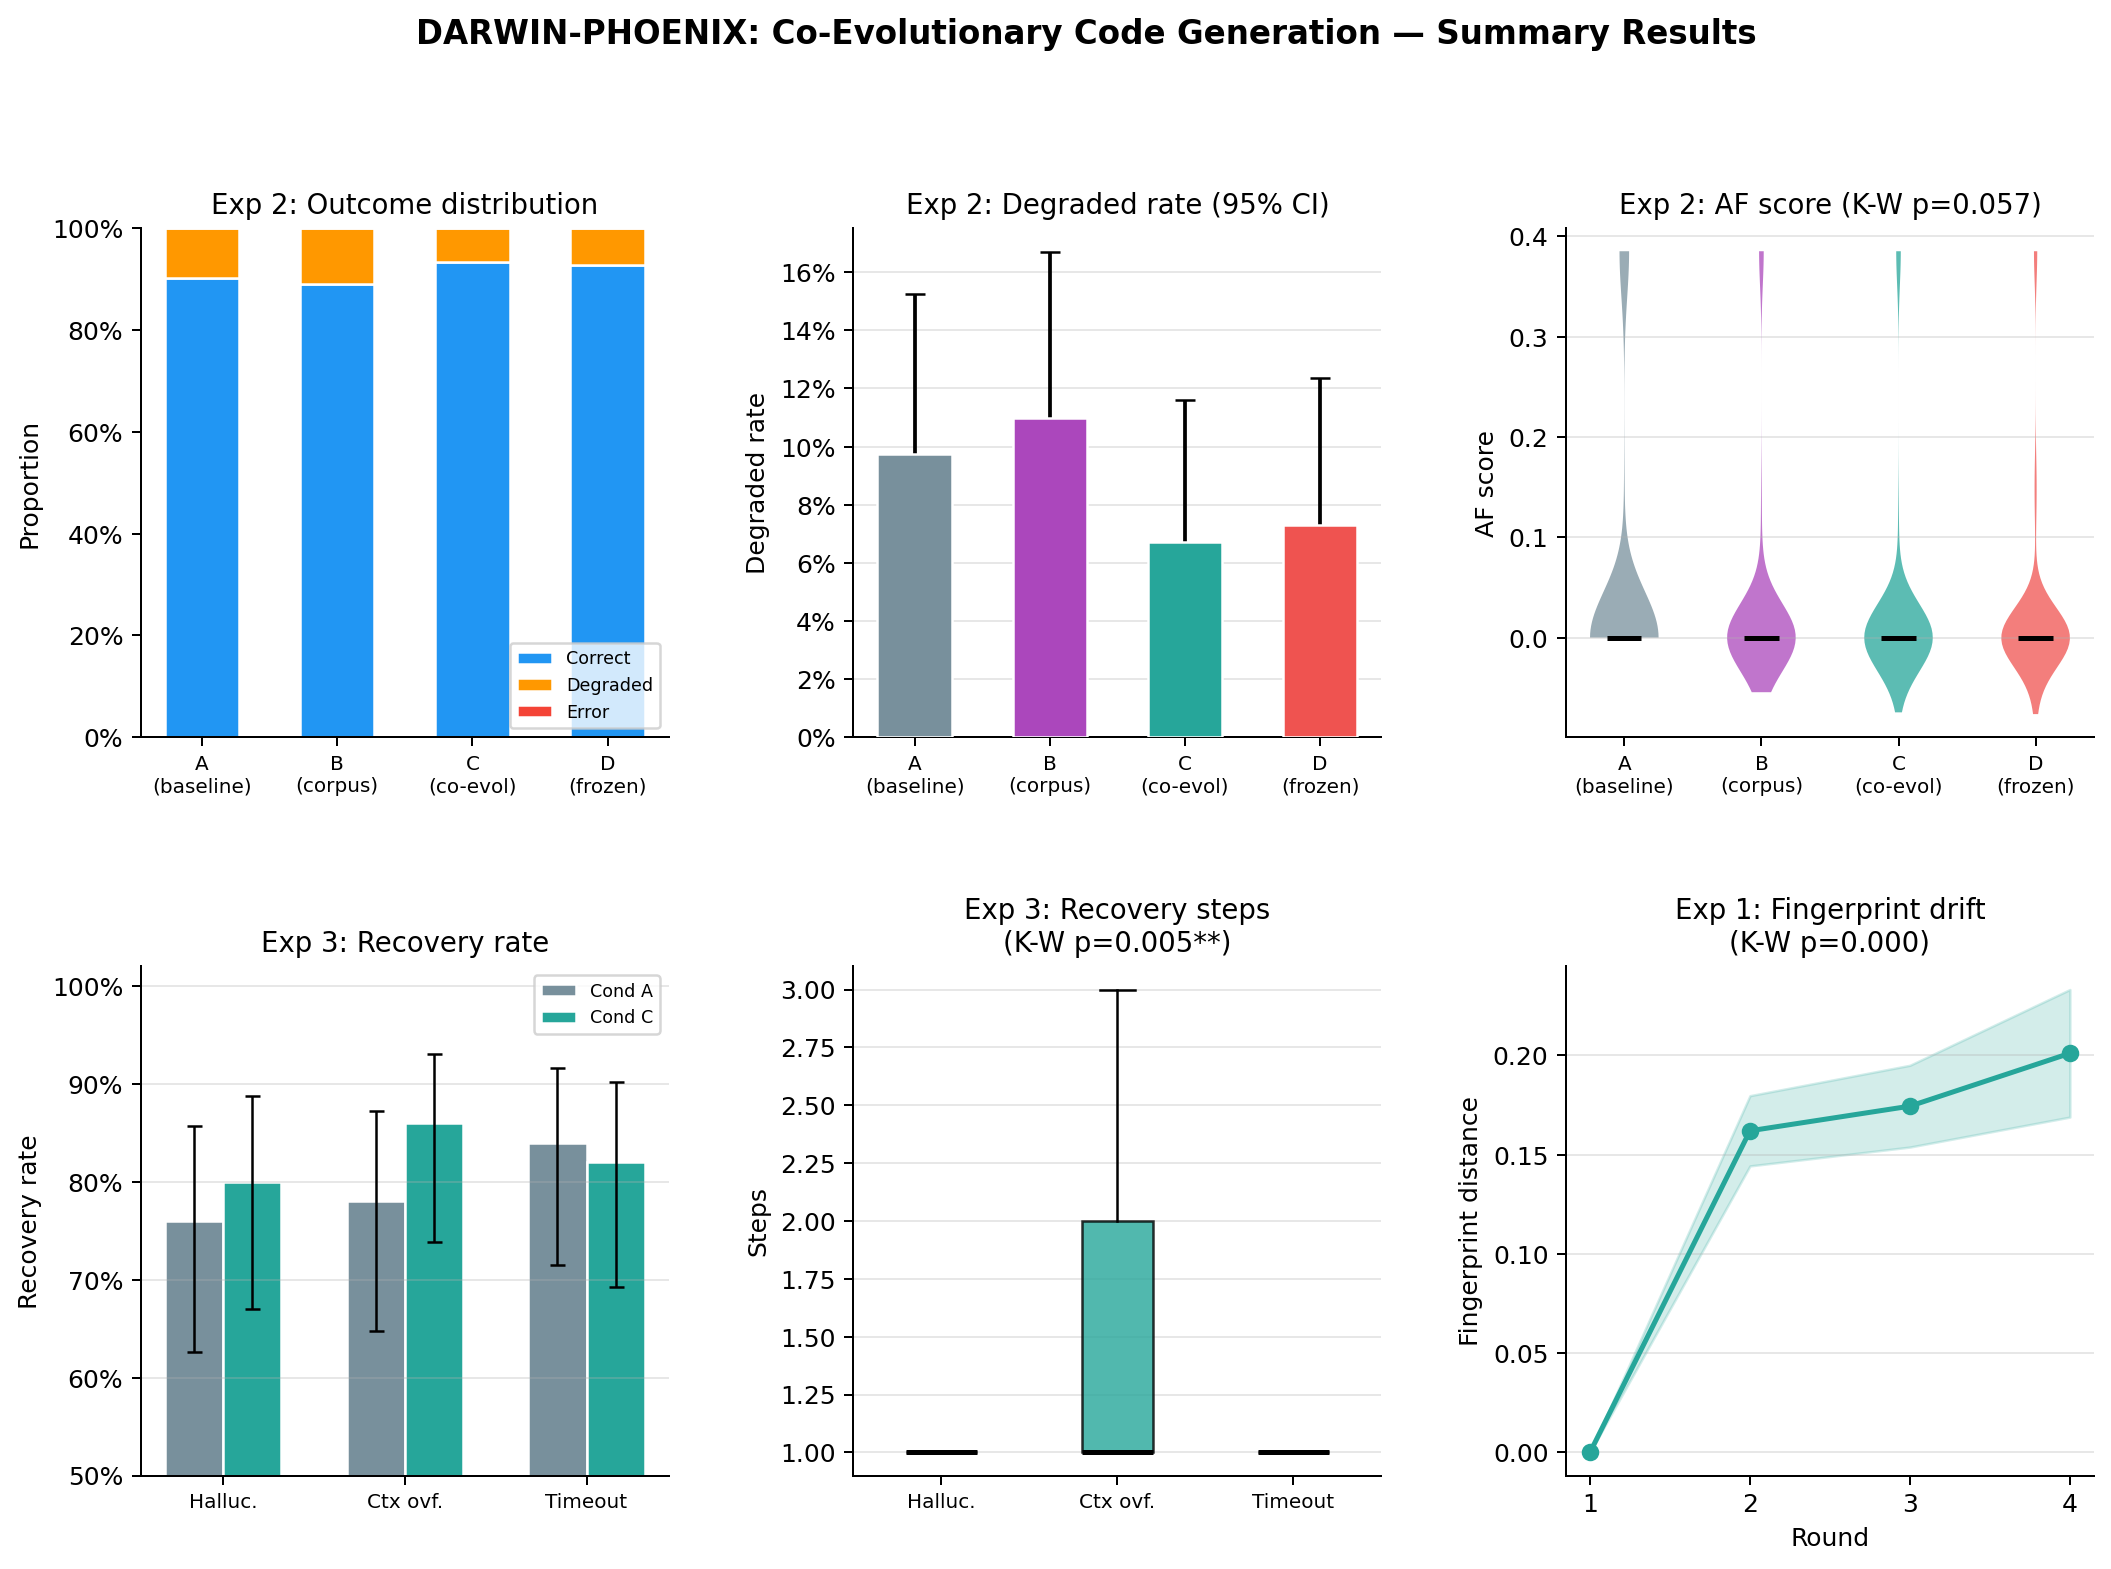
\includegraphics[width=0.95\linewidth]{figures/fig4_summary.png}
  \caption{Combined one-page summary across all three experiments.}
  \label{fig:summary}
\end{figure}

\section{Reproducibility}

\begin{itemize}
  \item \textbf{Code:} All experimental code in \texttt{experiments/} directory.
  \item \textbf{Data:} Results CSVs at \texttt{results/exp\{1,2,3\}\_results.csv}.
  \item \textbf{LLM:} Generator + Breaker: Qwen3-32B via OpenRouter
        (\texttt{qwen/qwen3-32b}). Evolver: Llama-3.1-8B-Instant via OpenRouter
        (\texttt{meta-llama/llama-3.1-8b-instant}).
  \item \textbf{Framework:} LangGraph~0.x, Python~3.13, scikit-learn (TF-IDF),
        scipy (statistics).
  \item \textbf{Benchmark:} HumanEval+ via \texttt{evalplus} library.
  \item \textbf{Hardware:} Windows~11, consumer-grade laptop, sequential/parallel
        API calls.
\end{itemize}

\section{Statistical Details}

Full statistical reports are provided in the accompanying repository
(\url{https://github.com/sakethyalamanchili/DARWIN-PHOENIX}):
\begin{itemize}
  \item \texttt{results/exp1\_statistical\_report.txt}
  \item \texttt{results/exp2\_statistical\_report.txt}
  \item \texttt{results/exp3\_statistical\_report.txt}
\end{itemize}

Key tests: Fisher exact (one-sided), Kruskal-Wallis, Mann-Whitney~U,
Spearman correlation, Cohen's~$h$, Wilson confidence intervals.

\end{document}
